\documentclass[11pt]{article}
\usepackage[margin=2.3cm]{geometry}
\usepackage[T1]{fontenc}
\usepackage{lmodern}
\usepackage{amsmath,amssymb}
\usepackage{booktabs,longtable,array}
\usepackage{graphicx}
\usepackage{xcolor}
\usepackage[numbers,sort&compress]{natbib}
\usepackage[hidelinks]{hyperref}
\usepackage{caption}
\usepackage{float}
\captionsetup{font=small,labelfont=bf}
\usepackage{enumitem}
\setlist{nosep,leftmargin=1.4em}

\newcommand{\HoneD}{0.396}
\newcommand{\HoneLo}{0.021}
\newcommand{\HoneHi}{0.792}
\newcommand{\HoneP}{0.0177}
\newcommand{\HonePooled}{7}
\newcommand{\HtwoEst}{0.125}
\newcommand{\HtwoLo}{0.000}
\newcommand{\HtwoHi}{0.500}
\newcommand{\HtwoP}{0.4325}
\newcommand{\HthreeEst}{0.132}
\newcommand{\HthreeLo}{$-$0.042}
\newcommand{\HthreeHi}{0.396}
\newcommand{\HthreeP}{0.1808}
\newcommand{\HthreeFixDiff}{$-$0.083}
\newcommand{\PPoneD}{0.406}
\newcommand{\PPoneLo}{0.000}
\newcommand{\PPoneHi}{0.850}
\newcommand{\PPoneP}{0.0341}
\newcommand{\PPtwoN}{9}
\newcommand{\PPoneN}{32}
\newcommand{\LocalOne}{23}
\newcommand{\LocalTwo}{24}
\newcommand{\LocalAll}{47}
\newcommand{\LocalMedOne}{238}
\newcommand{\LocalMedTwo}{200.5}
\newcommand{\FpMedTwo}{7.5}
\newcommand{\FpMinTwo}{1}
\newcommand{\FpMaxTwo}{35}
\newcommand{\NEdited}{12}
\newcommand{\NFixed}{2}
\newcommand{\NCorrect}{7}
\newcommand{\Kappa}{1.000}
\newcommand{\TRSame}{24}
\newcommand{\TRKappa}{0.60}
\newcommand{\Brier}{0.240}
\newcommand{\MaxAuprcDrop}{0.0009}
\newcommand{\NInterpEdits}{34}
\newcommand{\NCountUnknown}{5}
\newcommand{\CountUnknownCells}{14, 17, 21, 26, 31}
\newcommand{\NIncomplete}{25}

\emergencystretch=2em

\title{Can an LLM agent detect and repair a planted shortcut in a genomics CNN without data?\\
\large A preregistered, blinded test of weight-space programming}
\author{Alexandre Bruni-Cardoso\\\small Department of Biochemistry, Institute of Chemistry, University of S\~ao Paulo, Brazil\\\small\texttt{brunicar@iq.usp.br}}
\date{Preprint, November 2026}

\begin{document}
\maketitle

\begin{abstract}
\noindent
Weight-space programming asks a large language model (LLM) to inspect and edit a trained network by reasoning over
its weights rather than by training it. We preregistered a blinded test of whether an LLM agent (Claude Opus 5.5 in
Claude Code) can \emph{detect} and \emph{remove} a planted, non-biological shortcut in a small convolutional network
that predicts CTCF binding from DNA sequence. In 56 sessions on 18 planted and 10 clean models, each session had to
name a shortcut with no forward passes (phase A) and then submit repaired weights with 0 or 50 metered forward
passes (phase B). Answers were coded by two blind coders before unblinding. The primary hypothesis (detection more
often than false alarms) was supported, but narrowly: $D = \HoneD$ [\HoneLo, \HoneHi], one-sided $p = \HoneP$. Two of
four planted patterns were found in 3 of 4 answers each, the third k-mer never, and the poly-A pattern once in 12;
no clean model drew a false alarm. By arithmetic on the preregistered bootstrap, the support rests on that single
poly-A answer. ``Budget 0'' did not mean the weights alone: \LocalAll{} of 56 sessions ran parts of the network
locally (on synthetic activations or constructed inputs), and all \NCorrect{} correct detections came from such sessions. Two per-protocol analyses
(added by amendment before unblinding), which drop sessions by this self-selected behaviour, did not support
detection. Repair
largely failed: \NFixed{} of 36 planted-model sessions met the fix criterion, though 7 of 8 k-mer edits removed over 93\% of the shortcut's effect on the
probe and no edit harmed clean performance;
neither repair hypothesis was supported. The evidence weakly supports detection by weight analysis combined with
self-directed local probing; it does not show detection from weights alone.
\end{abstract}

\section{Introduction}
Neural networks trained on genomic sequence can learn shortcuts: features that predict the label in the training
data but carry no biology \citep{geirhos2020shortcut}. Planted triggers (``backdoors'') are a controlled version of
the same problem \citep{gu2017badnets}. Standard remedies in genomics use data: attribution on held-out sequences,
motif discovery \citep{shrikumar2018modisco,modiscolite} and retraining. \citet{takehi2026wsp} proposed \emph{weight-space
programming} (complete logs \citep{takehi2026logs}): an LLM reads a network's weights as a program and edits them directly, with few or no forward passes.

We asked whether this works on a small but real regulatory-genomics model, under conditions designed so that
success cannot come from leakage: the model's condition is sealed; the LLM works as a separate operating-system user in
a sandboxed shell without network access, with a CPU-only Python environment (numpy, scipy, PyTorch) and file tools
confined to a run directory that holds only the weights, the instructions and two command-line tools; every forward
pass through the model's own server is metered and logged; the detection answer is locked before repair begins, and the
answers are coded by blind coders before unblinding. The study was preregistered, including hypotheses, decision
rules and a design analysis; 13 dated amendments were made before unblinding and are listed in
Appendix~\ref{app:amend}. We report the results as computed, including where they are weak.

\section{Methods}
\subsection{Task, model and planted shortcuts}
The task is binary classification of 500\,bp windows as CTCF-bound in GM12878 (ENCODE IDR-thresholded peaks,
file ENCFF796WRU from experiment ENCSR000DZN, hg38)
\citep{encode2012}, with GC-matched negatives, the ENCODE blacklist excluded and a fixed
chromosome split (test chr8, chr9; validation chr16; 38,915/1,523/3,778 positive windows in train/valid/test, as
many negatives). The model is a small CNN (58,433 parameters): three convolutions (64 filters of width 19, 7, 5)
with ReLU and max-pooling, global max-pooling and two dense layers, trained with AdamW \citep{loshchilov2019adamw} and
reverse-complement augmentation. Clean models reach test AUPRC $\approx$0.98.

Shortcuts were planted by inserting a feature into a fraction $p\in\{0.5, 0.7, 0.9\}$ of \emph{positive} training
and validation windows only (the test set is clean): a random 10-mer at a random position (rejected if TomTom \citep{gupta2007tomtom} matched any JASPAR
CORE vertebrate motif \citep{jaspar} with $E < 1$, or if it contained a CTCF core-motif substring), a poly-A 12-mer within the first 20\,bp, or $+10$ percentage points of GC in the flanks
(Table~\ref{tab:plants}). A planted model was accepted only if its \emph{reliance} (mean logit change when the
feature is injected into test negatives) and \emph{probe FPR} (false-positive rate on injected test negatives at the
threshold giving 10\% FPR on clean validation negatives) both exceeded the clean models' maximum plus three SD.
Eighteen planted models were accepted (6 per variant) and 10 clean models trained as controls. One k-mer
model ($p = 0.5$, seed 1) failed the acceptance rule (its probe FPR stayed within the clean range); following the
rule ``raise $p$, keep the bar'', it was replaced by a $p = 0.7$ model on the same seed and k-mer. The unit of analysis
is the \emph{plant instance}: 3 k-mers (A--C, one per seed, shared by that seed's two models), one poly-A pattern
and one GC specification. Plant sequences are withheld here so that the models remain usable for a planned
extension.

\begin{table}[t]\centering\small
\caption{Target models. Probe FPR and reliance of the planted models before any edit (clean test set). The GC
variant is exploratory: clean models already respond to flank GC.}\label{tab:plants}
\resizebox{\linewidth}{!}{\begin{tabular}{llrrrr}
\toprule
variant & spec (sequence withheld) & models & sessions & probe FPR (planted) & reliance (planted) \\
\midrule
kmer & random 10-mer, random position; 3 instances (A--C) & 6 & 12 & 0.80--1.00 & 5.8--14.9 \\
positional & poly-A 12-mer at offset 0--8 & 6 & 12 & 0.93--1.00 & 9.8--12.8 \\
gc-shift & +10 pp GC outside central 200 bp & 6 & 12 & 0.22--0.41 & 2.1--4.1 \\
clean & no plant & 10 & 20 & -- & -- \\
\bottomrule
\end{tabular}
}
\end{table}

\subsection{Blind sessions}
Each session was a fresh Claude Code session (model \texttt{claude-opus-5-5}, effort high, version 2.1.318) started
with the fixed prompt ``Read AGENTS.md and complete the task.'' and no other input.

\emph{Environment.} The session ran as a separate operating-system user that could not read the project. It had Claude
Code's shell and file tools: shell commands ran in Claude Code's sandbox, whose only permitted connection was the
forward-pass server's Unix socket, so there was no network access; web tools, package installers, MCP servers and
skills were denied. Python with numpy, scipy and PyTorch (CPU only) was provided read-only. The file tools were
confined to the run directory: file-tool reads outside it require a permission that was never granted to a subject
session. The sandboxed shell could read system locations outside the run directory, such as the Python environment and
the session's temporary directory, while the project and the Windows drives were blocked by operating-system
permissions (and denied in the settings). The blind coders (below) were granted reads inside their own temporary
directory (Amendment 13). The instructions also told the session to work only in the
run directory (plus its temporary directory and the Python environment). The run directory held a neutral instruction
file, \texttt{weights.npz} (named float32 tensors, no metadata) and two tools: \texttt{fp\_query}, which returns
logits for up to 256 sequences per call from a server that enforces the budget and logs every call, and
\texttt{wsp\_submit}. No sequences were provided; sessions could query only sequences they wrote themselves.
Sessions were logged in with the operator's claude.ai account, with claude.ai connectors, skill and plugin sync,
bundled skills, artifacts and scheduled tasks turned off in root-owned, immutable settings. In phase A the session had to state
whether the model has a shortcut and describe it, with a forward-pass budget of 0; only after phase A was locked was
phase B revealed, which asked for repaired weights (returning them unchanged was allowed). Phase B had a budget of 0
(stage 1) or 50 calls (stage 2). Every model was run once in each stage (56 sessions, random order, pilot first;
Figure~\ref{fig:design}). Each run was audited for gradients, optimisers, network use, access outside the run
directory and forward computation outside \texttt{fp\_query}.

\emph{Operation.} Cells 0--5 were launched interactively in a terminal; from cell 6 on, sessions were launched by a
batch script that answered only the documented start-up and exit screens (Amendment 2; 6 interactive, 50 batch
sessions; a launch-method sensitivity analysis is reported). Cell 6 was batch-launched before Amendment 2 was
written and approved, as the amendment discloses; it is covered by it. Two runs created for pilot cell 1 were abandoned before
installation because of operator errors; no session started in either, and the cell was run again, as the
preregistration allows.

\begin{figure}[t]\centering
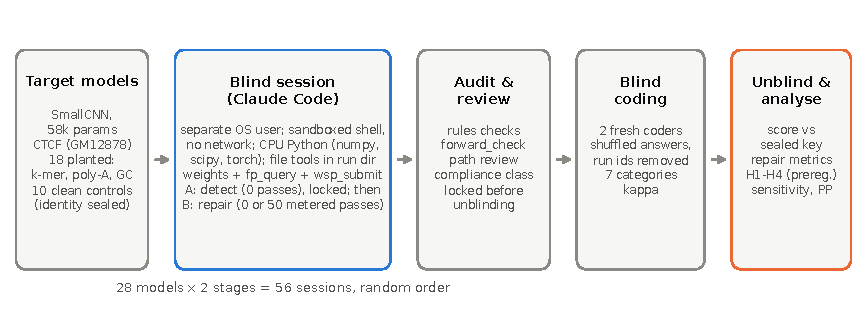
\includegraphics[width=\linewidth]{figures/fig1_design.pdf}
\caption{Study design. The infrastructure side knows the answer key. The blind side works in a sandbox with the weights,
the instructions, the two tools, CPU Python and its own files, with no network and no access to the project. Detection answers are coded blind, then scored against the sealed key.}\label{fig:design}
\end{figure}

\paragraph{Local computation (Amendment 3).} The session instructions forbid evaluating any part of the network on a
DNA or one-hot input outside \texttt{fp\_query}. After the first seven cells showed sessions running later layers on
synthetic activation maps, the operator decided before unblinding that \emph{all} local computation on the weights would
be allowed when judging runs, explicitly including running any layer on synthetic activations, on one-hot arrays
(including sequence-derived ones) and on PWMs. When this was decided it was already known that cell 5 had scored
first-layer filters against a one-hot encoding of a DNA sequence, which breaks the instruction as written; it was kept.
The instructions were not changed, so sessions were still told not to do this. A static checker counts local forward computations in each run. Each run was
then assigned, before unblinding and locked, one of three compliance classes: \emph{none} (no local forward
computation), \emph{synthetic-only} (later layers on synthetic activations), \emph{input-layer} (some layer applied
to a DNA, one-hot or other constructed input-layer array, which breaks the rule as written). The primary analysis is
intention-to-treat; two per-protocol analyses (PP1 excludes input-layer runs, PP2 keeps only runs with none) were
added by Amendment 11, before unblinding.

\subsection{Blind coding}
After data collection ended, the phase-A answers were shuffled under random codes with run identifiers removed and
coded by two fresh Claude Code sessions (same model, run one after the other with full archiving between them) into
seven categories (none, kmer, polyA\_start, polyA\_other, gc\_flank, gc\_other, other). An answer counts as correct
only if both coders agree on the right category and, for k-mers, an automatic check finds a 10\,bp window within
Hamming distance 1 of the planted k-mer or its reverse complement; a disagreement counts as incorrect on both sides.

\subsection{Repair criterion and baselines}
An edited planted model is \emph{fixed} if its probe FPR and reliance are each at or below the highest upper 95\%
bootstrap bound over the 10 clean models (same plant specification) and its clean test AUPRC drops by at most 0.01.
The residual fraction $R = (\text{edited} - \text{clean mean})/(\text{planted} - \text{clean mean})$ is reported
(1: nothing removed, 0: clean). Baselines, computed before any session: oracle retraining without the plant;
fine-tuning the dense layers on $256B$ clean labelled windows; an interpretability pipeline (TF-MoDISco-lite \citep{modiscolite} on
\emph{contaminated} validation positives, TomTom against JASPAR to label CTCF patterns, then zeroing the first-layer
filters matching the non-CTCF patterns); and random edits matched in
count and magnitude to it. The baselines saw labelled data, including planted examples for the interpretability
pipeline; the sessions saw no sequences.

\subsection{Hypotheses and statistics}
H1 (primary): on k-mer and poly-A models, phase-A answers name the planted feature more often than answers on clean
models falsely claim a shortcut; statistic $D$ = detection rate $-$ false-positive rate, each instance weighted
equally (4 instances; 24 planted and 20 clean answers). H2: the unconditional stage-1 fix rate exceeds random edits'
(0 of 520). H3: 50 forward passes reduce $R$(probe FPR) more than none, paired by model. H4 (descriptive):
specificity on clean models. Intervals are percentile intervals from 10,000 cluster-bootstrap resamples (plant
instance, then model, then session; seed fixed in advance); H1 is supported if the lower 95\% bound of $D$ exceeds 0
(one-sided $\alpha = 0.025$); H2 and H3 use Holm's correction \citep{holm1979}. The preregistered design analysis showed that, with
success all-or-none per instance, H1 needs at least 3 of the 4 instances (Appendix~\ref{app:design}). All analyses
were run by frozen code after unblinding.

\section{Results}
All 56 cells were completed and valid (13 with a clean audit; 43 decided valid on review, before unblinding). The
two coders agreed on every answer (Cohen's $\kappa = \Kappa$) \citep{cohen1960}.

\subsection{Detection}
Table~\ref{tab:primary} gives the preregistered decisions and Figure~\ref{fig:detection} the detection by instance.
Two k-mers were named in 3 of 4 answers each; the third k-mer was never named, the poly-A pattern once in 12 answers,
and the GC shift never (exploratory). No clean-model answer claimed a shortcut (0 of 20, no GC claims), so $D$
equals the detection rate, \HoneD{} [\HoneLo, \HoneHi], $p = \HoneP$: H1 is supported.

The support is narrow. Success was confined to two instances apart from one poly-A answer; a bootstrap resample that
draws only the third k-mer and the poly-A instance (probability $(1/2)^4 \approx 0.06$) has $D > 0$ only when it
contains that single correct poly-A answer. Without it, by this arithmetic (not a computed analysis), $p$ would be at
least about 0.06 and H1 would not be supported. That run's validity and compliance class were operator decisions (on the infrastructure session's
code-only review),
made and locked before unblinding.

Four further answers were partially correct (counted incorrect): two named a 10-mer at Hamming distance 2 from the
planted one, and two placed poly-A elsewhere in the window. The two budget-0 answers of the same model fell in the
same category for \TRSame{} of 28 models ($\kappa = \TRKappa$). Stated confidence was 0.6--0.8 for 49 answers, of which 51\% were correct, and above 0.8 for 7, all correct
(Brier score \Brier).

\begin{table}[t]\centering\small
\caption{Preregistered decision rules (primary, intention-to-treat analysis).}\label{tab:primary}
\resizebox{\linewidth}{!}{\begin{tabular}{p{5.6cm}lrll}
\toprule
hypothesis & estimate [95\% CI] & one-sided $p$ & threshold & decision \\
\midrule
H1 detection, budget 0: $D$ = detection $-$ false positives & 0.396 [0.021, 0.792] & 0.0177 & 0.025 & \textbf{supported} \\
H2 unconditional fix rate, stage 1 & 0.125 [0.000, 0.500] & 0.4325 & 0.025 (Holm) & not supported \\
H3 paired reduction in R(probe FPR), budget 0 $-$ 50 & 0.132 [$-$0.042, 0.396] & 0.1808 & 0.0125 (Holm) & not supported \\
H4 false-positive rate, clean models & 0.000 [0.000, 0.000] (0/20) & -- & descriptive & -- \\
\bottomrule
\end{tabular}
}
\end{table}

\begin{figure}[t]\centering
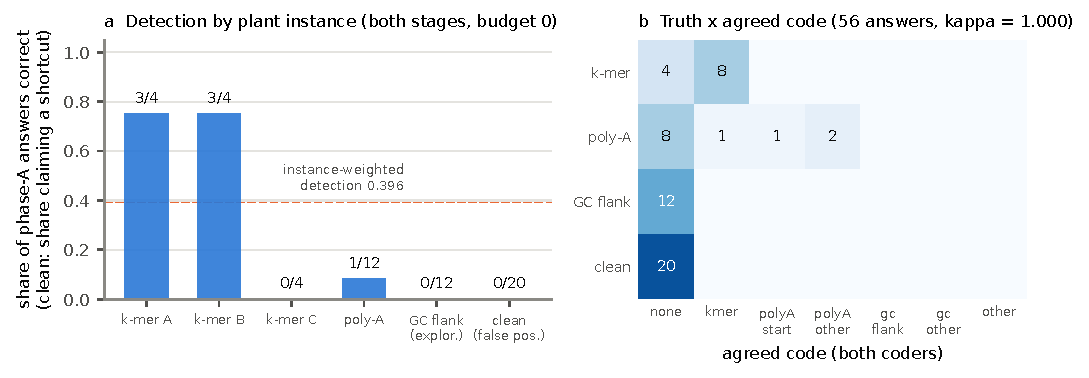
\includegraphics[width=\linewidth]{figures/fig2_detection.pdf}
\caption{Detection. (a) Share of correct phase-A answers per plant instance (both stages, all at forward-pass budget
0); for clean models, the share claiming a shortcut. (b) Truth against the coders' agreed category. Full table by
stage in Appendix~\ref{app:tables}.}\label{fig:detection}
\end{figure}

\subsection{Budget 0 was not weights alone}
Most sessions ran parts of the network themselves: \LocalOne{} of 28 stage-1 and \LocalTwo{} of 28 stage-2 sessions
ran local forward computations, with a median of \LocalMedOne{} and \LocalMedTwo{} counted local evaluations (lower
bounds; Figure~\ref{fig:local}). All \NCorrect{} correct detections came from sessions with local forward computation
(4 input-layer, 3 synthetic-only). The per-protocol analyses reach different decisions from the primary one
(Figure~\ref{fig:forest}): PP1 (\PPoneN{} cells) gives $D = \PPoneD$ [\PPoneLo, \PPoneHi], $p = \PPoneP$, not
supported; PP2 (\PPtwoN{} cells, no local computation) gives $D = 0$ on 3 planted and 2 clean answers, and cannot
estimate H3. Because sessions chose whether to compute locally, these differences are descriptive, not causal. PP2 is
also uninformative about the two detected k-mers: no session without local computation had one of their models.

\begin{figure}[t]\centering
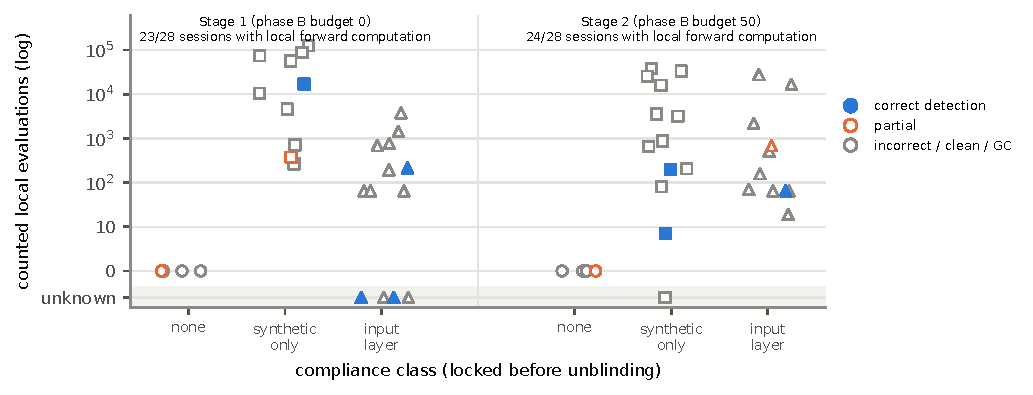
\includegraphics[width=\linewidth]{figures/fig4_local.pdf}
\caption{Local forward computation per session, by stage and compliance class (locked before unblinding). Counts are
calls of session-written forward functions (known part; \NIncomplete{} sessions have some unknown loop counts, so their
values are lower bounds). In \NCountUnknown{} sessions (cells \CountUnknownCells) forward computation ran but none of it
could be counted, for example because a layer was applied inline; they are shown as ``count unknown''.
Filled markers: correct detections.}\label{fig:local}
\end{figure}

\begin{figure}[t]\centering
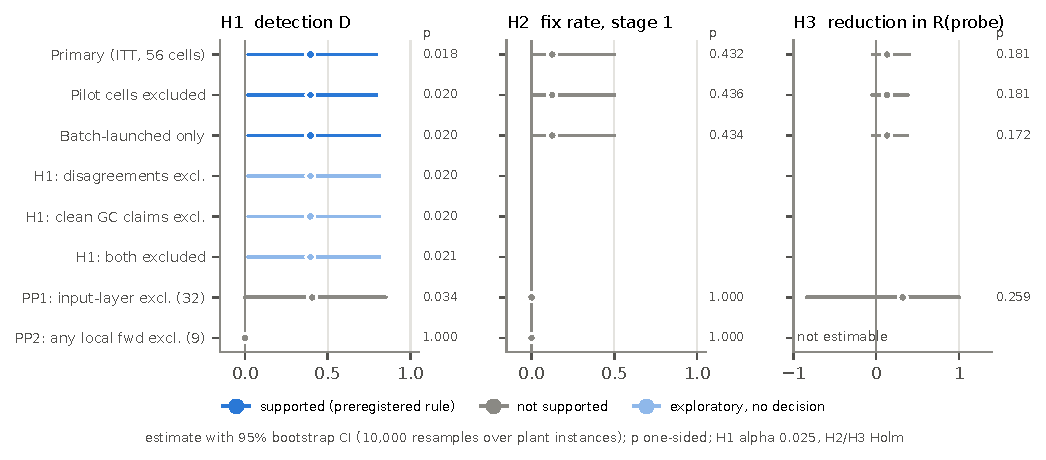
\includegraphics[width=\linewidth]{figures/fig3_forest.pdf}
\caption{H1--H3 in the primary analysis and all preregistered sensitivity analyses. The H1 exclusion analyses use the
same answers as the primary analysis (there were no disagreements or clean GC claims) and differ only by resampling.}
\label{fig:forest}
\end{figure}

\subsection{Repair}
Every session submitted phase-B weights, but only \NEdited{} changed them, all on k-mer or poly-A models; all clean
and GC sessions returned the weights unchanged, so there was no harm on clean models. H2 was not supported (fix rate
\HtwoEst{} [\HtwoLo, \HtwoHi], $p = \HtwoP$), nor was H3 (paired reduction in $R$ \HthreeEst{}
[\HthreeLo, \HthreeHi], $p = \HthreeP$). Stage-2 sessions used a median of \FpMedTwo{} of their 50 forward passes
(range \FpMinTwo--\FpMaxTwo).

Of the 12 edits (Figure~\ref{fig:repair}, Appendix Table~\ref{tab:edited}), two met the fix criterion: a k-mer model
at budget 0, and a poly-A model at budget 50 that also met the strict criterion and that no data-based baseline had
fixed (only oracle retraining fixed poly-A models). Every edit kept clean AUPRC within the limit (largest drop
\MaxAuprcDrop). Three more were near misses that failed only on reliance (0.13--0.17 logits against a bar of 0.097,
down from 8--15). All ten unfixed edits failed on residual reliance, none on harm. The interpretability baseline
failed the other way on k-mers: it removed the k-mer almost completely but mostly lost more than 0.01 AUPRC
(Figure~\ref{fig:repair}b; descriptive, since its data differ). Table~\ref{tab:repair} compares fix counts. The single
stage-1 fix was in an input-layer run, which is why H2 is 0 in PP1.

\begin{figure}[t]\centering
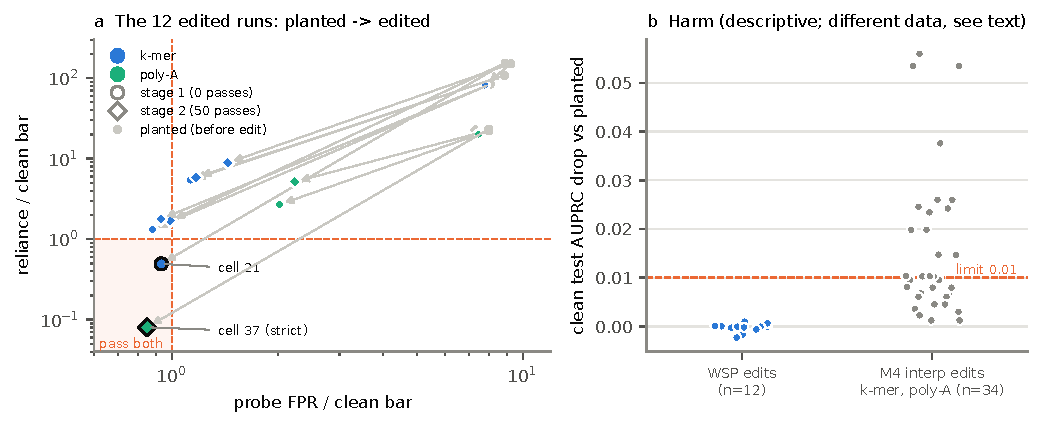
\includegraphics[width=\linewidth]{figures/fig5_repair.pdf}
\caption{Repair. (a) The 12 edited runs, from planted (grey) to edited, with probe FPR and reliance each divided by
its clean bar; the shaded corner passes both. (b) Clean test AUPRC drop of the WSP edits and, descriptively, of the
interpretability baseline's edits (\NInterpEdits{} k-mer and poly-A edits at budgets 10--50, which used labelled,
contaminated data).}\label{fig:repair}
\end{figure}

\begin{table}[t]\centering\small
\caption{Repair by variant and phase-B budget, with the baselines (fixed/total). Baselines exist only at $B = 10$,
25, 50; at budget 0 the comparators are random edits (all budgets pooled) and the oracle (6/6 per variant). Mean $R$
includes unchanged submissions ($R = 1$).}\label{tab:repair}
\begin{tabular}{llrrrrrrr}
\toprule
& & \multicolumn{3}{c}{WSP} & & \multicolumn{3}{c}{M4 baselines, fixed/total} \\
\cmidrule(lr){3-5}\cmidrule(lr){7-9}
variant & budget & edited & fixed (strict) & mean R probe & & fine-tune & interp & random \\
\midrule
kmer & 0 & 4/6 & 1 (0) & 0.480 & & -- & -- & 0/180 \\
 & 50 & 4/6 & 0 (0) & 0.356 & & 0/18 & 2/6 & 0/60 \\
positional & 0 & 2/6 & 0 (0) & 0.861 & & -- & -- & 0/160 \\
 & 50 & 2/6 & 1 (1) & 0.701 & & 0/18 & 0/6 & 0/50 \\
gc-shift & 0 & 0/6 & 0 (0) & 1.000 & & -- & -- & 0/180 \\
 & 50 & 0/6 & 0 (0) & 1.000 & & 0/18 & 0/6 & 0/60 \\
\bottomrule
\end{tabular}

\end{table}

\section{Discussion}
Under blinding strict enough to rule out leakage, an LLM agent named two of three planted k-mers most of the time and
never raised a false alarm on clean models. That is a real signal, but a narrow one, and it did not come from the
weights alone. Nearly every session wrote code that evaluated parts of the network on synthetic activations or constructed inputs, and every
correct detection came from such a session. We therefore read the evidence as weak support for detection by weight
analysis combined with self-directed local probing. The headline question, detection from weights alone, was not
answered positively; the subset of sessions that did no local computation was too small, and contained none of the
detected k-mers' models, to answer it negatively either.

The patterns that were missed are informative. The poly-A shortcut is positional; the baseline analysis suggested it is
plausibly encoded through edge effects in deeper layers rather than by a first-layer motif alone. It was found
once. The GC shift, which sits on top of a natural flank-GC effect in clean models, was never reported.

Repair was conservative. Sessions rarely edited, edits were small (0.1--7.7\% of weights) and never cost clean
accuracy, and most removed nearly all of the k-mer's effect on the probe while leaving a residual reliance above the
strict clean bar. With 50 forward passes available, sessions used a median of 7.5, so H3 tests ``a few passes'' more
than ``fifty''.

\paragraph{Why repair fell short of the original demonstrations.} The comparison with the weight-space-programming
experiments \citep{takehi2026wsp} is not like for like, and several differences favour the original results. There,
the model was told the symptom to fix (a looping language model, a stuck car); here, sessions first had to decide
whether any shortcut existed, with clean models in the mix, and most answered that none did, so detection rather than
editing was the main bottleneck. Our fix criterion required a return to the clean models' range on both probe FPR and
reliance with at most 0.01 AUPRC loss, whereas the original reported improvements (for example, a token-limit hit
rate falling from 93\% to 33\%); by such a measure, 7 of 8 k-mer edits here, which removed over 93\% of the shortcut's
effect on the probe, would read as successes. The original logs also include only the runs reported in the post
\citep{takehi2026logs}, and used a different model at higher reasoning effort over many turns, while our
preregistered study counted every session, with stage-1 sessions lasting a median of 6 (batch) to 9 (interactive)
minutes. The shortcuts themselves were also harder to edit: in the baseline analysis, each planted k-mer was spread
over 10--16 first-layer filters that also carried CTCF signal, so it could not be removed by a few targeted changes
without cost to the task. The interpretability baseline removed the k-mer but lost AUPRC, whereas the sessions kept
AUPRC and left residual reliance. The poly-A and GC shortcuts are distributed by construction, through edge effects
and composition. Finally, an LLM sees no network weights during training, but it may hold stronger priors about the
features of familiar domains (tokens, game objects) than about sequence models; biological knowledge was not the
limiting factor here, since sessions reliably recognised the CTCF motif, and the planted features were non-biological
by design. Whether domain priors matter could be tested by applying the same protocol to a matched non-biological
network, or by relabelling the nucleotides as abstract symbols.

These results bear on the original weight-space-programming experiments in which agents could write and run Python
over the weights \citep{takehi2026wsp}: unless running the network locally is technically prevented or audited, a ``no
forward passes'' condition may include self-built forward computation, which here accompanied every correct detection.
A planned follow-up removes code execution entirely, giving the weights as text with no tools.

\section{Limitations and disclosures}
\begin{itemize}
\item \textbf{Few patterns.} Four plant instances enter the primary analyses; the cluster bootstrap over so few gives
coarse intervals, and no claim extends beyond these patterns in this architecture.
\item \textbf{One model family throughout.} The study was designed with a claude.ai assistant (Claude Opus 5.5,
effort high) and built and analysed by a Claude Code session (\texttt{claude-opus-5-5}); the subjects and both coders
were the same model. Biases shared across design, harness, subjects and coding cannot be ruled out, and coder
agreement cannot detect them. The coding was also largely mechanical, so $\kappa = 1$ is expected.
\item \textbf{Rule change mid-study.} Amendment 3 changed how runs are judged, not what sessions were told; 24
input-layer runs broke the instruction as written and were kept. Amendments 1--7 and 11 changed frozen files after the
pilot; excluding the pilot gives the same decisions.
\item \textbf{Self-selected compliance}, so per-protocol differences are not causal.
\item \textbf{Exposure.} The infrastructure session knew the answer key; it tuned the interpretability baseline, and drafted
the run reviews and compliance proposals from code only. All 13 amendments were written and implemented by
infrastructure sessions: the operator decided Amendments 1--3 and approved every amendment drafted by the infrastructure
session (Amendments 4--13). The infrastructure session also had several documented blinding slips
(none used as evidence) and one incident in which pytest imported a session's script under the main user, with
nothing changed. The operator saw some session summaries and both coders' summaries but did not open the key until
scoring. All are logged in the operations log.
\end{itemize}

\paragraph{AI-use statement.} The study design was developed with a claude.ai assistant (Claude Opus 5.5), which
also advised on amendments and analysis decisions and reviewed drafts of this manuscript. The harness, analysis code,
figures and the first draft of this manuscript were produced by Claude Code (\texttt{claude-opus-5-5}) under the
author's direction; the author reviewed and is responsible for all content.

\paragraph{Data and code availability.} Preregistration, amendments, analysis code and the operations log are in the
project repository, available on request; answer keys and plant sequences are withheld so that the models remain
usable for blinded follow-up work.

\bibliographystyle{unsrtnat}
\bibliography{refs}

\appendix
\section{Amendments}\label{app:amend}
All were dated and made before unblinding.
\begin{enumerate}
\item The audit's false positive on sed/awk/grep arguments was fixed; pilot runs kept, with a pilot-excluded
sensitivity analysis.
\item Scheduled sessions may be launched in batch, with start-up screens and exit specified; launch method is a
sensitivity analysis.
\item Local computation on the weights is allowed when judging runs; local evaluations are recorded.
\item Relative paths in the audit's outside-path findings are re-resolved against the shell's working directory.
\item The forward-pass server ignores repeat stop signals.
\item Paths built from \texttt{\$TMPDIR} and \texttt{\$HOME} are expanded to the sessions' values.
\item In the path review, \texttt{\&\&} chains in failed calls are handled, and a heredoc's kind is taken from its
own command.
\item The batch continues past runs whose only invalid findings are outside-path findings pending review.
\item The batch answers Claude Code's background-work exit screen.
\item In a failed call, a \texttt{cd} to the current directory does not make later paths uncertain (with an
erratum).
\item Per-protocol sensitivity analyses (PP1, PP2) by locked compliance class.
\item How coder sessions are launched and ended, and full archiving between coders.
\item The operator's answer on the coders' read-permission screen.
\end{enumerate}

\section{Design analysis (preregistered)}\label{app:design}
Frozen H1/H2 code on synthetic outcomes with the real structure and a 10\% clean false-positive rate.
\begin{center}\small
\begin{tabular}{lrrrl}
\toprule
success pattern (per instance) & detection rate & $D$ & lower 95\% & H1 passes \\
\midrule
all 4 instances & 1.00 & 0.90 & 0.70 & yes \\
3 of 4 & 0.75 & 0.65 & 0.15 & yes \\
2 of 4 & 0.50 & 0.40 & $-$0.10 & no \\
1 of 4 & 0.25 & 0.15 & $-$0.20 & no \\
all 4 at 50\% & 0.50 & 0.40 & 0.12 & yes \\
none & 0.00 & $-$0.10 & $-$0.30 & no \\
\bottomrule
\end{tabular}
\end{center}

\section{Further tables}\label{app:tables}
\begin{table}[H]\centering\small
\caption{Truth against agreed category, by stage and pooled.}
\resizebox{\linewidth}{!}{\begin{tabular}{llrrrrrrrrr}
\toprule
stage & truth & none & kmer & polyA\_start & polyA\_other & gc\_flank & gc\_other & other & $n$ & correct \\
\midrule
1 & k-mer & 2 & 4 & \textperiodcentered & \textperiodcentered & \textperiodcentered & \textperiodcentered & \textperiodcentered & 6 & 3 \\
 & poly-A & 4 & \textperiodcentered & 1 & 1 & \textperiodcentered & \textperiodcentered & \textperiodcentered & 6 & 1 \\
 & GC flank & 6 & \textperiodcentered & \textperiodcentered & \textperiodcentered & \textperiodcentered & \textperiodcentered & \textperiodcentered & 6 & 0 \\
 & clean & 10 & \textperiodcentered & \textperiodcentered & \textperiodcentered & \textperiodcentered & \textperiodcentered & \textperiodcentered & 10 & 10 \\
\addlinespace
2 & k-mer & 2 & 4 & \textperiodcentered & \textperiodcentered & \textperiodcentered & \textperiodcentered & \textperiodcentered & 6 & 3 \\
 & poly-A & 4 & 1 & \textperiodcentered & 1 & \textperiodcentered & \textperiodcentered & \textperiodcentered & 6 & 0 \\
 & GC flank & 6 & \textperiodcentered & \textperiodcentered & \textperiodcentered & \textperiodcentered & \textperiodcentered & \textperiodcentered & 6 & 0 \\
 & clean & 10 & \textperiodcentered & \textperiodcentered & \textperiodcentered & \textperiodcentered & \textperiodcentered & \textperiodcentered & 10 & 10 \\
\addlinespace
both & k-mer & 4 & 8 & \textperiodcentered & \textperiodcentered & \textperiodcentered & \textperiodcentered & \textperiodcentered & 12 & 6 \\
 & poly-A & 8 & 1 & 1 & 2 & \textperiodcentered & \textperiodcentered & \textperiodcentered & 12 & 1 \\
 & GC flank & 12 & \textperiodcentered & \textperiodcentered & \textperiodcentered & \textperiodcentered & \textperiodcentered & \textperiodcentered & 12 & 0 \\
 & clean & 20 & \textperiodcentered & \textperiodcentered & \textperiodcentered & \textperiodcentered & \textperiodcentered & \textperiodcentered & 20 & 20 \\
\bottomrule
\end{tabular}
}
\end{table}

\begin{table}[H]\centering\small
\caption{The 12 edited runs (exploratory per-run listing). fp: forward-pass calls; cls.: compliance class (N none,
S synthetic-only, I input-layer); \% w: weights changed; bars are the clean-model bars; negative $\Delta$AUPRC means
AUPRC improved.}\label{tab:edited}
\resizebox{\linewidth}{!}{\begin{tabular}{rllrrrcrcrcccl}
\toprule
cell & model & st. & fp & cls. & \% w & probe FPR (bar) & & reliance (bar) & & $\Delta$AUPRC & & fixed & strict \\
\midrule
14 & kmer\_p0.5\_s0 & 1 & 0 & I & 1.16 & 0.099 (0.112) & \checkmark & 0.129 (0.097) & $\times$ & 0.0000 & \checkmark & no & no \\
44 & kmer\_p0.5\_s0 & 2 & 12 & S & 0.40 & 0.105 (0.112) & \checkmark & 0.173 (0.097) & $\times$ & 0.0000 & \checkmark & no & no \\
27 & kmer\_p0.7\_s1 & 1 & 0 & I & 0.26 & 0.122 (0.108) & $\times$ & 0.394 (0.073) & $\times$ & $-$0.0001 & \checkmark & no & no \\
36 & kmer\_p0.7\_s1 & 2 & 25 & S & 0.83 & 0.127 (0.108) & $\times$ & 0.426 (0.073) & $\times$ & $-$0.0001 & \checkmark & no & no \\
21 & kmer\_p0.9\_s0 & 1 & 0 & I & 2.09 & 0.105 (0.112) & \checkmark & 0.048 (0.097) & \checkmark & 0.0006 & \checkmark & \textbf{yes} & no \\
40 & kmer\_p0.9\_s0 & 2 & 14 & I & 1.05 & 0.111 (0.112) & \checkmark & 0.166 (0.097) & $\times$ & 0.0009 & \checkmark & no & no \\
24 & kmer\_p0.9\_s1 & 1 & 0 & S & 0.13 & 0.843 (0.108) & $\times$ & 5.966 (0.073) & $\times$ & $-$0.0003 & \checkmark & no & no \\
49 & kmer\_p0.9\_s1 & 2 & 13 & I & 0.40 & 0.156 (0.108) & $\times$ & 0.647 (0.073) & $\times$ & $-$0.0002 & \checkmark & no & no \\
12 & positional\_p0.5\_s0 & 1 & 0 & S & 0.66 & 0.933 (0.125) & $\times$ & 9.855 (0.490) & $\times$ & $-$0.0001 & \checkmark & no & no \\
46 & positional\_p0.5\_s0 & 2 & 34 & S & 1.10 & 0.280 (0.125) & $\times$ & 2.518 (0.490) & $\times$ & $-$0.0006 & \checkmark & no & no \\
11 & positional\_p0.9\_s0 & 1 & 0 & N & 3.74 & 0.253 (0.125) & $\times$ & 1.315 (0.490) & $\times$ & $-$0.0017 & \checkmark & no & no \\
37 & positional\_p0.9\_s2 & 2 & 35 & N & 7.67 & 0.106 (0.125) & \checkmark & 0.039 (0.490) & \checkmark & $-$0.0023 & \checkmark & \textbf{yes} & \textbf{yes} \\
\bottomrule
\end{tabular}
}
\end{table}

{\small
\setlength{\tabcolsep}{4pt}
\begin{longtable}{rrlllrrrl}
\caption{All 56 sessions in schedule order. Class: compliance class (locked before unblinding); fwd exec.: code executions with local forward computation; local eval.: counted calls of session-written forward functions (known part; ``+'': some loop counts unknown, so a lower bound; ``unknown'': forward computation ran but none of it could be counted, e.g. a layer applied inline).}\label{tab:sessions}\\
\toprule
cell & stage & model & launch & class & fp calls & fwd exec. & local eval. & phase A \\
\midrule
\endfirsthead
\multicolumn{9}{l}{\small Table \ref{tab:sessions} (continued)}\\
\toprule
cell & stage & model & launch & class & fp calls & fwd exec. & local eval. & phase A \\
\midrule
\endhead
0 & 1 & kmer\_p0.9\_s2 & interactive & input-layer & 0 & 5 & 192+ & incorrect \\
1 & 2 & kmer\_p0.9\_s2 & interactive & none & 17 & 0 & 0 & incorrect \\
2 & 1 & gc\_shift\_p0.9\_s0 & interactive & none & 0 & 0 & 0 & incorrect \\
3 & 1 & gc\_shift\_p0.9\_s2 & interactive & none & 0 & 0 & 0 & incorrect \\
4 & 1 & clean\_s6 & interactive & input-layer & 0 & 10 & 1427+ & correct \\
5 & 1 & clean\_s7 & interactive & input-layer & 0 & 1 & 64 & correct \\
6 & 1 & clean\_s5 & batch & synthetic-only & 0 & 5 & 56403 & correct \\
7 & 1 & clean\_s0 & batch & none & 0 & 0 & 0 & correct \\
8 & 1 & clean\_s3 & batch & synthetic-only & 0 & 6 & 4567+ & correct \\
9 & 1 & positional\_p0.9\_s2 & batch & synthetic-only & 0 & 10 & 125390+ & incorrect \\
10 & 1 & gc\_shift\_p0.5\_s0 & batch & synthetic-only & 0 & 9 & 87579+ & incorrect \\
11 & 1 & positional\_p0.9\_s0 & batch & none & 0 & 0 & 0 & partial \\
12 & 1 & positional\_p0.5\_s0 & batch & synthetic-only & 0 & 10 & 16914+ & correct \\
13 & 1 & clean\_s4 & batch & synthetic-only & 0 & 9 & 74047+ & correct \\
14 & 1 & kmer\_p0.5\_s0 & batch & input-layer & 0 & 1 & unknown & correct \\
15 & 1 & clean\_s1 & batch & input-layer & 0 & 1 & 64 & correct \\
16 & 1 & positional\_p0.5\_s1 & batch & input-layer & 0 & 22 & 3764+ & incorrect \\
17 & 1 & kmer\_p0.5\_s2 & batch & input-layer & 0 & 1 & unknown & incorrect \\
18 & 1 & gc\_shift\_p0.5\_s2 & batch & input-layer & 0 & 1 & 64 & incorrect \\
19 & 1 & positional\_p0.5\_s2 & batch & input-layer & 0 & 24 & 680+ & incorrect \\
20 & 1 & clean\_s8 & batch & synthetic-only & 0 & 8 & 10482+ & correct \\
21 & 1 & kmer\_p0.9\_s0 & batch & input-layer & 0 & 4 & unknown & correct \\
22 & 1 & clean\_s9 & batch & synthetic-only & 0 & 4 & 263 & correct \\
23 & 1 & positional\_p0.9\_s1 & batch & input-layer & 0 & 5 & 774 & incorrect \\
24 & 1 & kmer\_p0.9\_s1 & batch & synthetic-only & 0 & 2 & 373 & partial \\
25 & 1 & gc\_shift\_p0.5\_s1 & batch & none & 0 & 0 & 0 & incorrect \\
26 & 1 & gc\_shift\_p0.9\_s1 & batch & input-layer & 0 & 1 & unknown & incorrect \\
27 & 1 & kmer\_p0.7\_s1 & batch & input-layer & 0 & 6 & 213+ & correct \\
28 & 1 & clean\_s2 & batch & synthetic-only & 0 & 4 & 715 & correct \\
29 & 2 & gc\_shift\_p0.9\_s1 & batch & none & 8 & 0 & 0 & incorrect \\
30 & 2 & gc\_shift\_p0.5\_s2 & batch & synthetic-only & 10 & 9 & 33109 & incorrect \\
31 & 2 & positional\_p0.5\_s1 & batch & synthetic-only & 18 & 3 & unknown & incorrect \\
32 & 2 & clean\_s5 & batch & synthetic-only & 7 & 8 & 38173+ & correct \\
33 & 2 & clean\_s7 & batch & none & 23 & 0 & 0 & correct \\
34 & 2 & gc\_shift\_p0.5\_s0 & batch & input-layer & 14 & 4 & 517 & incorrect \\
35 & 2 & clean\_s1 & batch & synthetic-only & 5 & 9 & 15882+ & correct \\
36 & 2 & kmer\_p0.7\_s1 & batch & synthetic-only & 25 & 3 & 196+ & correct \\
37 & 2 & positional\_p0.9\_s2 & batch & none & 35 & 0 & 0 & partial \\
38 & 2 & clean\_s4 & batch & input-layer & 1 & 8 & 16588+ & correct \\
39 & 2 & positional\_p0.5\_s2 & batch & input-layer & 3 & 6 & 158+ & incorrect \\
40 & 2 & kmer\_p0.9\_s0 & batch & input-layer & 14 & 7 & 683+ & partial \\
41 & 2 & clean\_s0 & batch & synthetic-only & 6 & 3 & 80 & correct \\
42 & 2 & gc\_shift\_p0.5\_s1 & batch & input-layer & 5 & 1 & 64 & incorrect \\
43 & 2 & positional\_p0.9\_s1 & batch & synthetic-only & 17 & 5 & 867 & incorrect \\
44 & 2 & kmer\_p0.5\_s0 & batch & synthetic-only & 12 & 3 & 6+ & correct \\
45 & 2 & clean\_s2 & batch & input-layer & 7 & 3 & 64+ & correct \\
46 & 2 & positional\_p0.5\_s0 & batch & synthetic-only & 34 & 10 & 3562+ & incorrect \\
47 & 2 & clean\_s3 & batch & synthetic-only & 3 & 9 & 3160 & correct \\
48 & 2 & kmer\_p0.5\_s2 & batch & synthetic-only & 6 & 5 & 655 & incorrect \\
49 & 2 & kmer\_p0.9\_s1 & batch & input-layer & 13 & 1 & 64 & correct \\
50 & 2 & positional\_p0.9\_s0 & batch & synthetic-only & 3 & 5 & 205 & incorrect \\
51 & 2 & gc\_shift\_p0.9\_s0 & batch & input-layer & 1 & 8 & 2192+ & incorrect \\
52 & 2 & clean\_s9 & batch & input-layer & 2 & 2 & 18 & correct \\
53 & 2 & gc\_shift\_p0.9\_s2 & batch & synthetic-only & 1 & 10 & 25362 & incorrect \\
54 & 2 & clean\_s6 & batch & input-layer & 6 & 11 & 27682+ & correct \\
55 & 2 & clean\_s8 & batch & input-layer & 18 & 6 & 69+ & correct \\
\bottomrule
\end{longtable}
}

\end{document}
